\setlength{\parindent}{2em}

\section{Introduction}
\indent Certain physiological mechanisms that drive biological processes follow periodic synchronizations or rhythms. Examples of such phenomena include our heartbeats, the circadian rhythm, the menstrual cycle, hormone regulation, oscillating neurons, and more. While disruption or dis-regulation of proper biological rhythms has been associated with disease, induced perturbations to these oscillating systems (via a pacemaker or administration of therapeutic drugs) can reset the dynamics back to normal states\supercite{Glass2001}. 
\indent In 1994, Glass \& Sun\supercite{GLASS1994} mathematically approximated the effects of periodic pulsatile stimulations to cardiac oscillations using the Poincaré oscillator model. The oscillator is a 2D vector in an abstract  polar coordinate ($r$, $\phi$) state space with $0\leq \phi \leq 1$, that evolves with time according to:

\begin{align}
   \frac{\partial r}{\partial t} &= kr(1-r)\\ 
   \frac{\partial \phi}{\partial t}&=1
\end{align}

\noindent where $r$ is the radial coordinate, $\phi$ is the angular coordinate, and $k$ is the relaxation rate representing the rate of return to the circular limit cycle located at $r=1$. This evolution is periodically interrupted by a horizontal perturbation of magnitude $b$ every $\tau$ units of time. Initially, a point ($r_i$, $\phi_i$) is perturbed horizontally by an amount $b$ to ($r'_i$,$\phi'_i$), then ($r'_i$, $\phi'_i$) is evolved according to the differential equations above for a time $\tau$ arriving at the point ($r_{i+1}$, $\phi_{i+1}$) (see Fig \ref{osc}). We can solve these differential equations explicitly to get a 2-dimensional map relating the  perturbation points ($r'_i$,$\phi'_i$) to the next point at time $\tau$ after relaxation, $(r_{i+1}, \phi_{i+1})$.

\begin{equation}
    r_{i+1} = \frac{r'_i}{(1 - r'_i)e^{-k\tau}+r'_i}
    \label{eqn:1}
\end{equation}

\begin{equation}
    \textnormal{mod} \{\phi_{i+1} = \phi_i' + \tau,1\}
    \label{eqn:2}
\end{equation}

Glass \& Sun \supercite{GLASS1994} studied the organization of regions in (\emph{b}, $\tau$) space for which a stable periodic oscillation and fixed point exists. These regions, called phase-locking regions or "Arnold tongues", depend on the relaxation rate $\emph{k}$. They are annotated according to the number of stimuli per period (period \#) and the number of complete revolutions in phase (cycle \#) before returning to the fixed point $\phi$.

\begin{figure}[hbt!]
    \begin{center}
    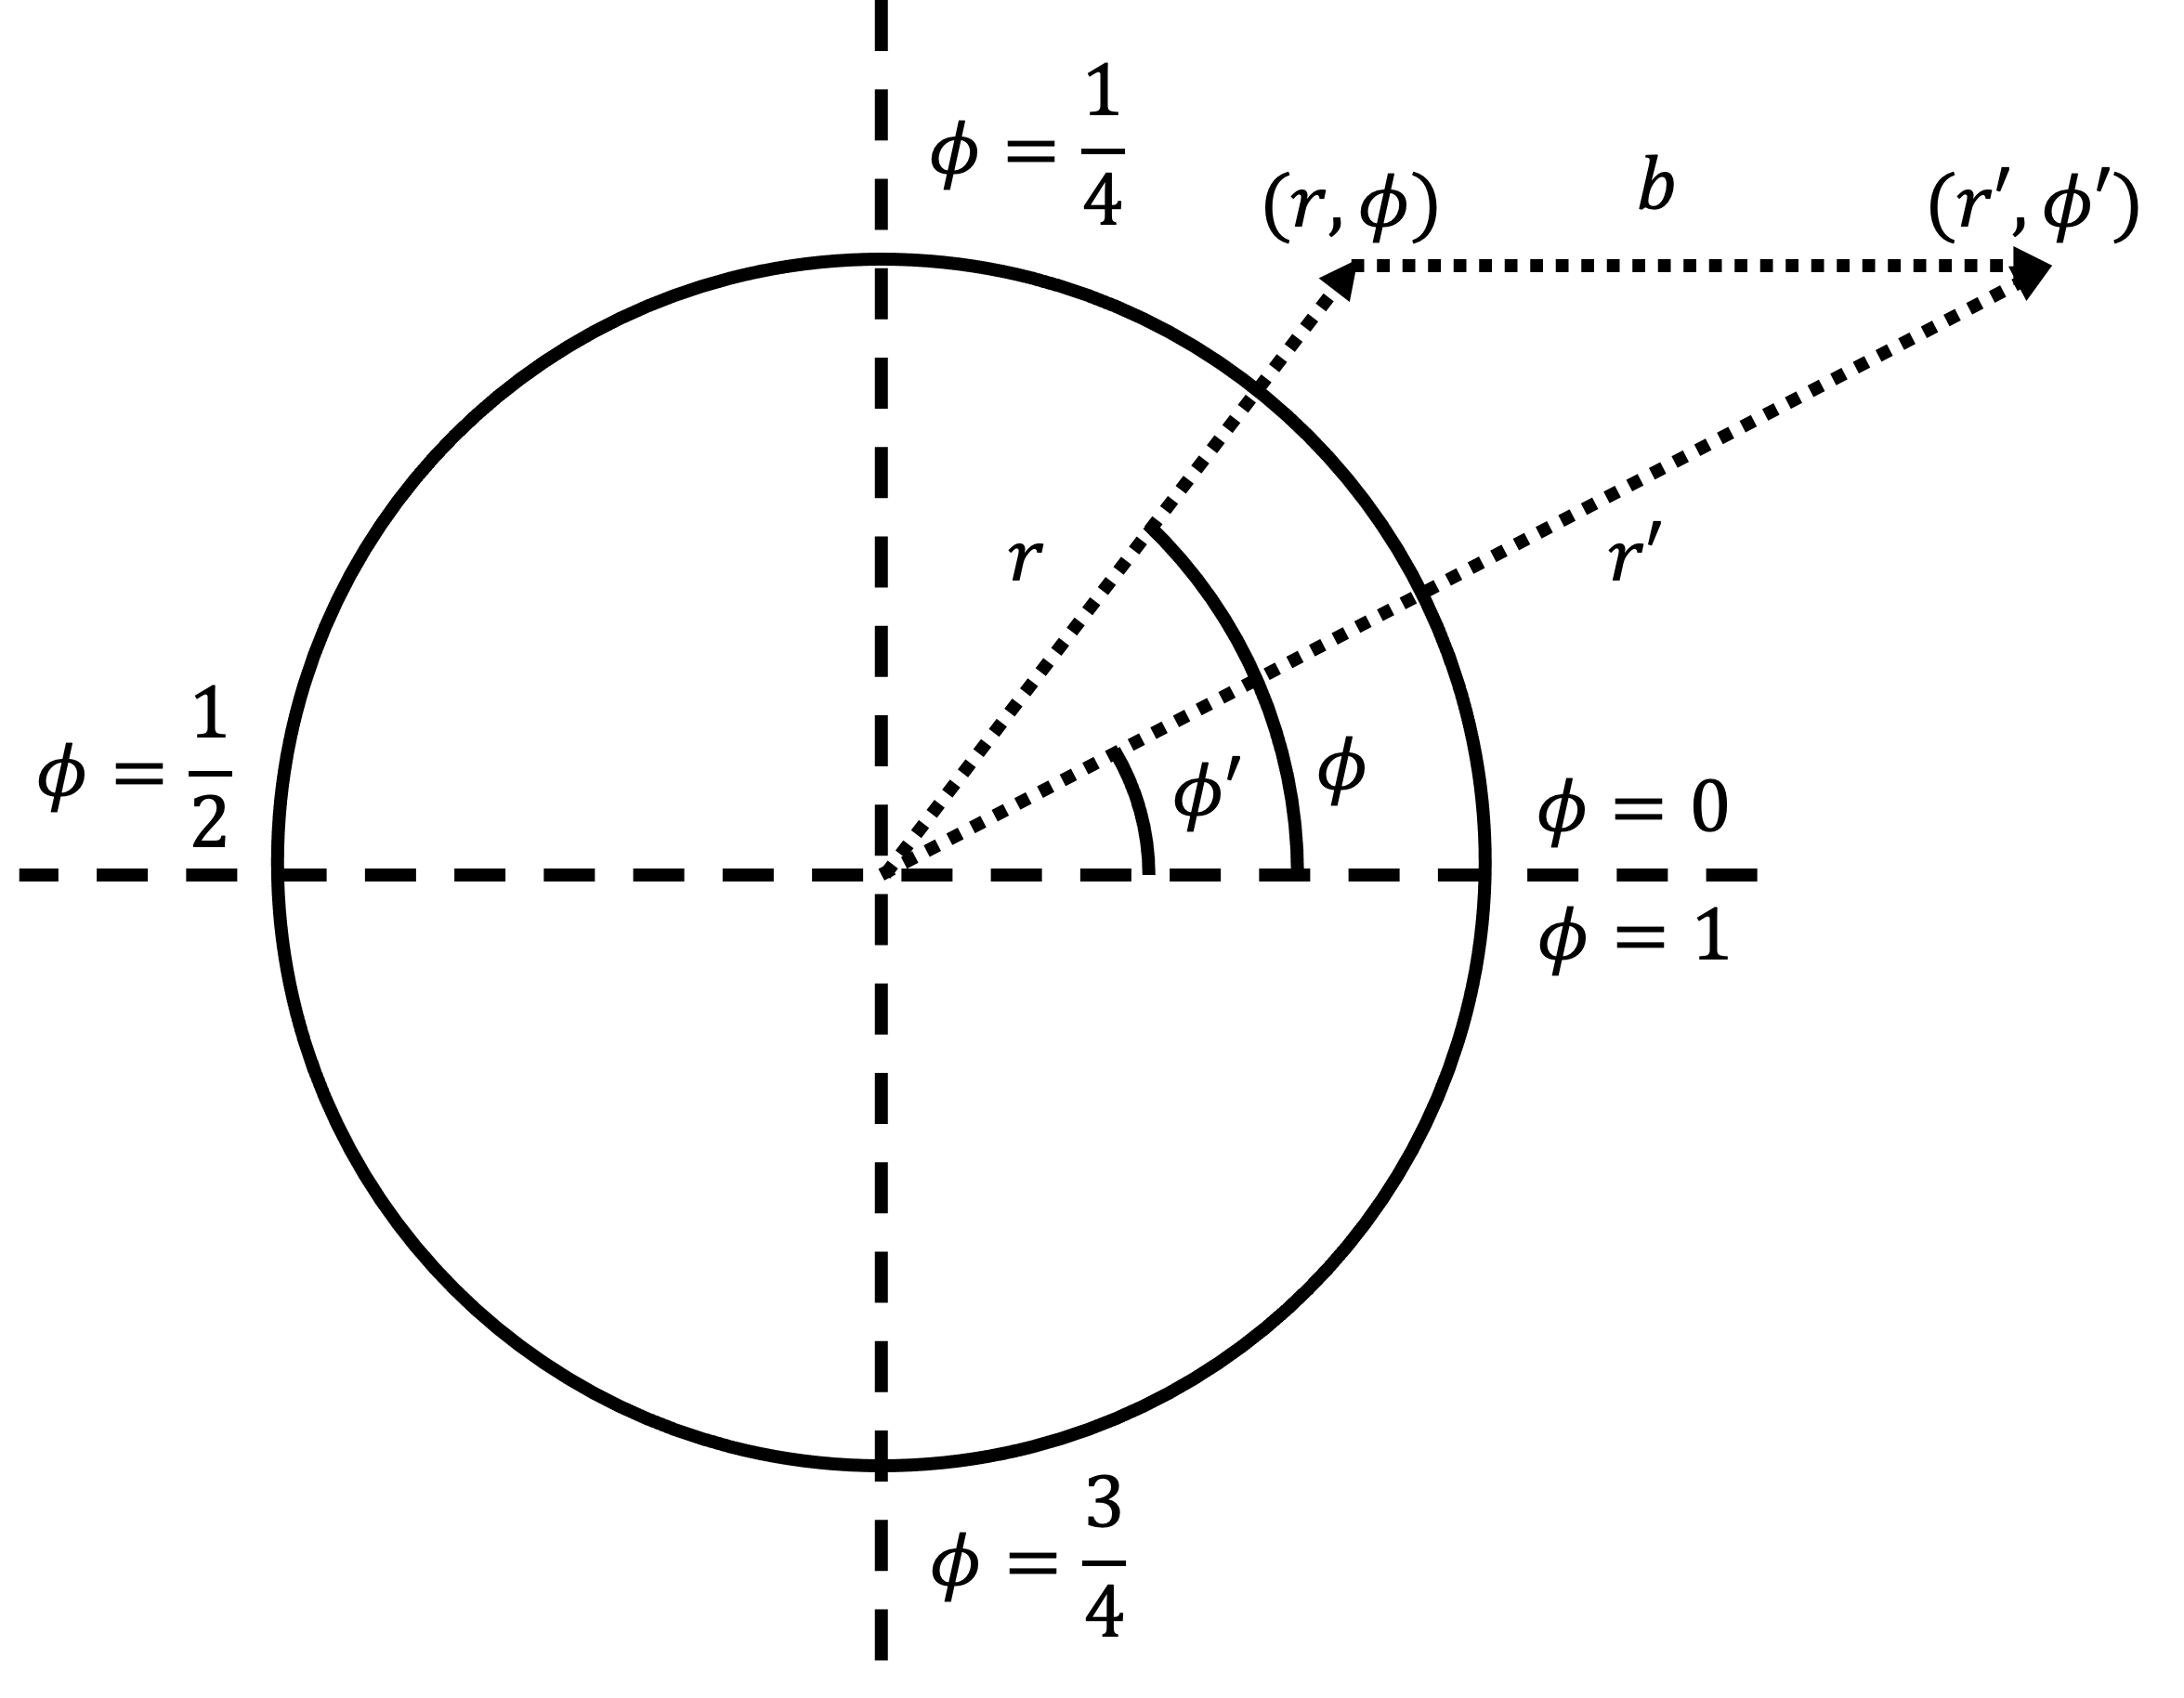
\includegraphics[width=.7\textwidth]{../plots/Fig1.png}
    \end{center}
    \caption{A diagram of the oscillator, as seen in Figure 1 from Glass \& Sun \cite{GLASS1994}.}
    \label{osc}
\end{figure}

\indent In this study, we successfully replicate the complex dynamical behaviour observed by Glass \& Sun (1994)\supercite{GLASS1994} resulting from only two uncoupled ordinary differential equations and periodic forcing. This replication study is significant because, firstly, it numerically describes how the finite relaxation rate back to the limit cycle affects the complex organization of the phase-locking regions and, secondly, because it analytically clarifies aspects of the instability boundary along the 1:0 and 1:1 (period \#: cycle \#) phase-locking regions in the infinite relaxation limit $(k \xrightarrow{} \infty$).

\section{Numerical Methods}
\label{sec: Numerical Methods}
\indent We successfully replicated the results of Glass \& Sun (1994)\supercite{GLASS1994} in the programming language Julia (version 1.7.2).
To overcome numerical inaccuracy issues, we use a version of the system\supercite{Glass2017} transformed into Cartesian coordinates with the form ($x_i$, $y_i$) using equations (\ref{eqn:1}) \& (\ref{eqn:2}):

\begin{equation}
    x_{i+1} = \frac{(x_i + b)\cos(2\pi\tau) - y_i \sin(2\pi\tau)}{(1 - r'_i)e^{-k\tau}+r'_i}
    \label{eqn:7}
\end{equation}

\begin{equation}
    y_{i+1} = \frac{y_i \cos(2\pi\tau) + (x_i + b) \sin(2\pi\tau)}{(1-r'_i)e^{-k\tau} + r'_i}
    \label{eqn:8}
\end{equation}

where

\begin{equation}
    r'_i = [(x_i + b)^2 + y^2_i]^{1/2} \nonumber 
\end{equation}

This resolves the issue of round-off errors when $r_i \approx 1$, $b \approx 1$, and $\phi_i \approx 0.5$. In order to visually compare our results with the original paper, we then convert the Cartesian coordinates back into Polar coordinates.

We use initial values ($x = 1$, $y = 0$) equivalent to ($r = 1$, $\phi = 0$) for $k=50\approx \infty$ to replicate Figure 2 of Glass \& Sun (1994)\supercite{GLASS1994}. The model is simulated over a period of 800 time-steps, however, we only consider the periodic cycles after a 500 transient time had passed.

We compare the global organization of phase-locking regions for different values of $b$ and $\tau$ at $k=50\approx \infty$, $k = 10$, and $k = 1$. For $k$ set as $10$ or $1$, we use the initial points ($x = -0.3081$, $y = 0.9514$) which correspond approximately to the arbitrarily chosen initial states ($r = 1$, $\phi = 0.3$) of the original paper. Furthermore, to investigate the dynamics at specific regions of the phase-locking zones, we produce Figures \ref{replic}d and \ref{replic}e, zoomed in at $\tau = 0.25$ and $b = 1$.

Figure \ref{replic} shows the phase-locking zones between the number of stimuli per period (denoted \emph{period n}) for 1 cycle, in an $n:1$ ratio. This differs from Glass \& Sun (1994)\supercite{GLASS1994} where $\tau$ was set between 0 and 2. We chose $\tau$ between 1 and 2 as it is simply a reflection of the image at $\tau$ between 0 and 1.

\begin{figure}[tbph]

\centering
        \subfloat[]{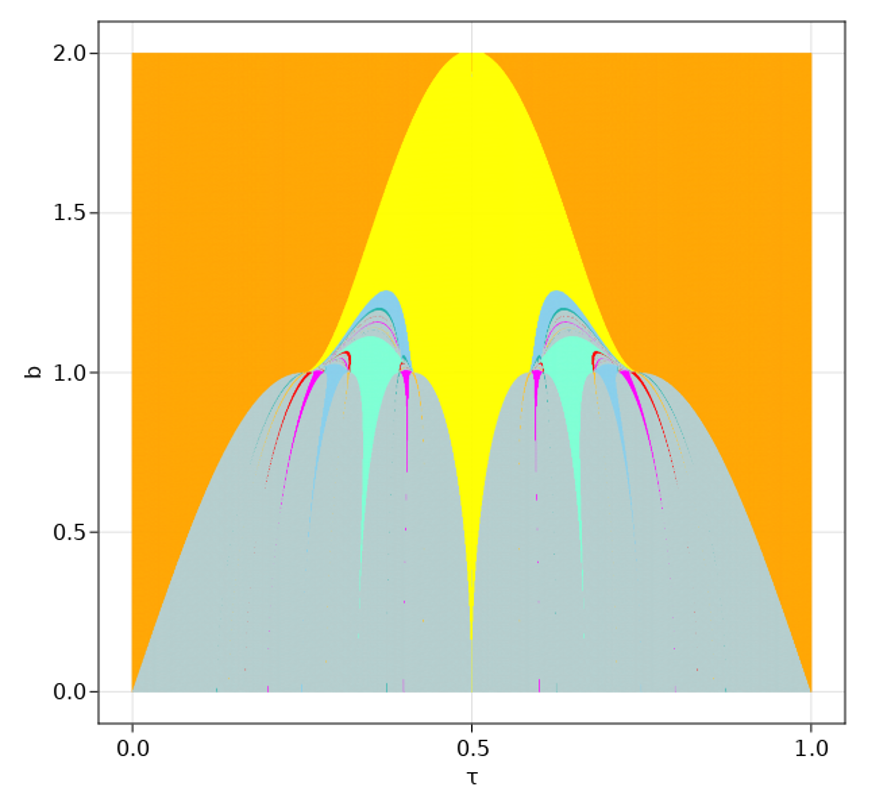
\includegraphics[width=0.45\textwidth]{../plots/k50_1.png}\label{fig:a}}
    \medskip
        \subfloat[]{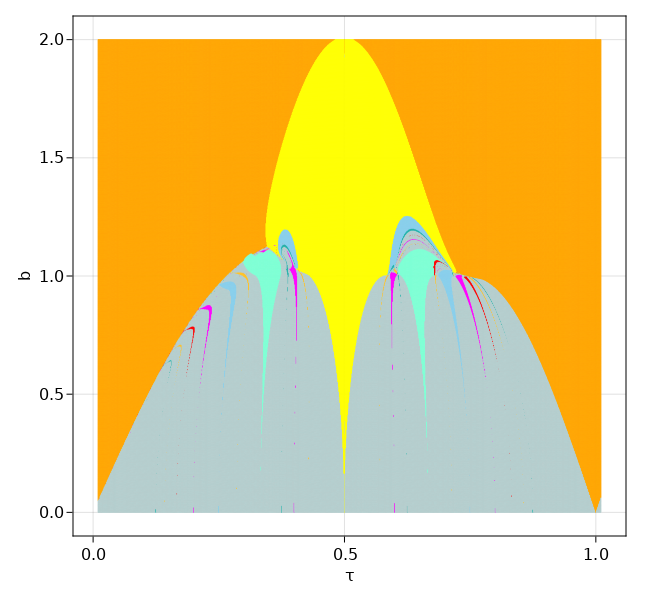
\includegraphics[width=0.45\textwidth]{../plots/k10.png}\label{fig:b}}
    \hfil
        \subfloat[]{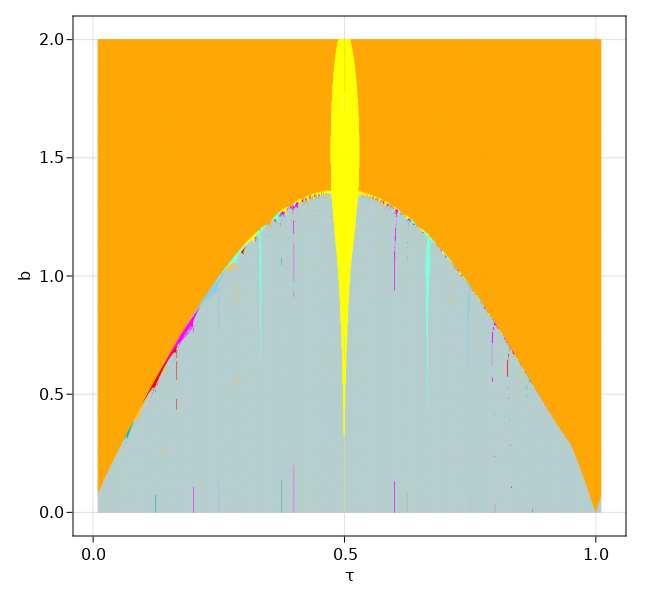
\includegraphics[width=0.45\textwidth]{../plots/k1.png}\label{fig:d}}
    \medskip
        \subfloat[]{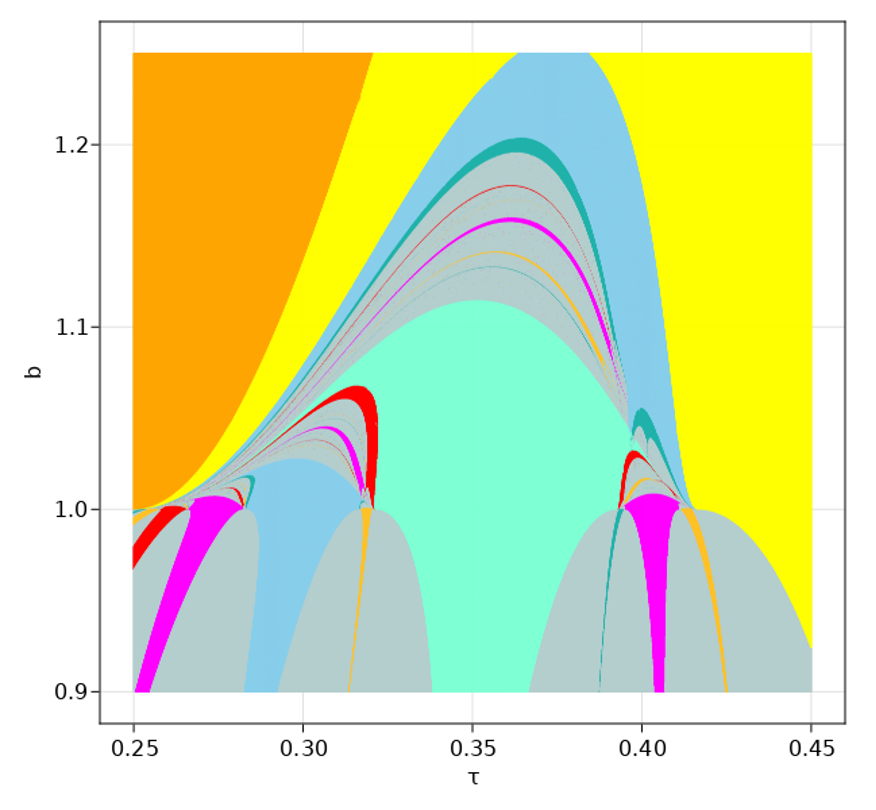
\includegraphics[width=0.45\textwidth]{../plots/k50_2.png}\label{fig:e}}
    \hfil
        \subfloat[]{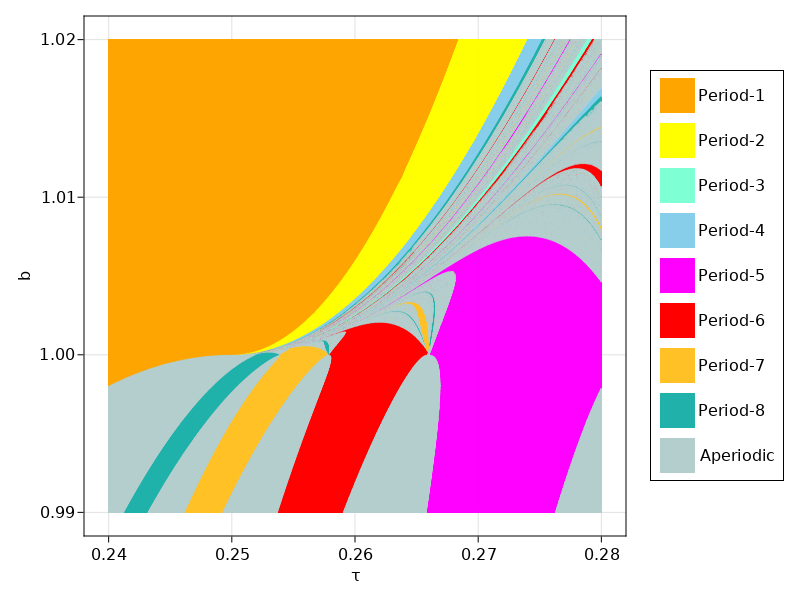
\includegraphics[width=0.6\textwidth]{../plots/zoom_zoom_plot.png}\label{fig:f}}
    
\caption{\textbf{Global organization of phase-locking zones of the periodically forced oscillator for different relaxation rate}. We demonstrate the organization of the phase-locking zones for (a) $k = 50 \approx \infty$; (b) $k = 10$; (c) $k = 1$; (d) $k = 50$ at increased resolution at point $\tau = 0.25$ and $b = 1.0$; (e) $k = 50$ at increased resolution at point $\tau = 0.35$ and $b = 1$. We show the $n:1$ locked period-cycles for different frequencies of stimulus $\tau$ and magnitude of stimulus $b$, as aforementioned in the text. We were able to successfully reproduce corresponding Figure 2, Figure 5a and Figure 5b of the original study. Despite the expected minor differences, our results follow the same overall patterns.}
    \label{replic}
\end{figure}

\section{Analytical Results}
\indent Here, we analytically calculate the period-1 instability boundary in the immediate relaxation limit ($k \rightarrow \infty$). $k \rightarrow \infty$ is called the immediate relaxation limit as the system returns (in the radial direction) to the limit cycle at $r=1$ immediately after the perturbation; all time evolutions occur on the unit circle and the 2D map reduces to a 1D map described by $\phi_{i+1}(\phi_i, b, \tau)$. The period-1 instability boundary is determined by setting $\phi_{i+1} = \textnormal{mod} \{\phi_i,1\}$ (period-1 condition, see equation \ref{eqn:2}) and $|\frac{\partial \phi_{i+1}}{\partial \phi_i}|>1$ (instability condition). $|\frac{\partial \phi_{i+1}}{\partial \phi_i}|>1$ represents small deviations from the fixed point becoming larger after applications of the 1D map (Strogatz, 2000\supercite{Strogatz}). After a few standard manipulations, as described in the Appendix section \ref{supp: sub1}, we find for the 1D map $\phi_{i+1}(\phi_i, b, \tau)$ the following result; and calculate its derivative.
\begin{equation}
    \phi_{i+1} =
    \begin{cases}
     \frac{1}{2\pi}\arccos(\frac{b+r \cos(\phi 2\pi)}{\sqrt{r^2+b^2+2rb\cos(\phi 2\pi)}}) + \tau & 0 \leq \phi_i \leq 1/2 \\
    -\frac{1}{2\pi}\arccos(\frac{b+r \cos(\phi 2\pi)}{\sqrt{r^2+b^2+2rb\cos(\phi 2\pi)}}) + 1 +\tau & 1/2 \leq \phi_i \leq 1 \\
    \end{cases}
    \label{eq: 1D map}
\end{equation} The derivative is found to be:
%derivative
\begin{equation}
    \frac{\partial \phi_{i+1}}{\partial \phi_i} = \frac{1+b\cos(2\pi \phi_i)}{1 + b^2 + 2b\cos(2\pi \phi_i)}
\end{equation}

\indent The general strategy to compute the instability is to set $\frac{\partial \phi_{i+1}}{\partial \phi_i} = \pm 1$ which will give an equation for $b(\phi_i)$. $b(\phi_i)$ can be substituted into $\phi_{i+1}(\phi_i,b,\tau)$; and setting $\phi_{i+1} = \phi_i$ (period-1 condition) gives $\phi_i(\tau)$. Finally, $\phi_i(\tau)$ is substituted into $b(\phi_i)$ resulting in the period-1 ($k\rightarrow \infty$) instability boundary $b(\tau)$.\\
We start by setting $\frac{\partial \phi_{i+1}}{\partial \phi_i} = 1$.
\begin{align}
    1 &= \frac{1+b\cos(2\pi \phi_i)}{1 + b^2 + 2b\cos(2\pi \phi_i)} \\
    b&= -\cos(2\pi \phi_i) \label{eq: bcos}
\end{align} This is then substituted in Eq. \ref{eq: 1D map}, and the period-1 condition is applied. 

\noindent For $0 \leq \phi_i \leq 1/2$, we have: \begin{align}
    \phi_{i+1} &= \phi_i = \frac{1}{2\pi}\arccos(\frac{b+\cos(\phi_i 2\pi)}{\sqrt{1+b^2+2b\cos(\phi_i 2\pi)}}) + \tau \\
    &= \frac{1}{2\pi}\arccos(0) + \tau = 1/4 +\tau.
\end{align} 
Since $1/4 + \tau = \phi_{i+1} = \phi_i \leq 1/2$, this implies $\tau \leq 1/4$.
    
\noindent For $1/2 \leq \phi_i \leq 1$, we have:
\begin{align}
    \phi_{i+1} &= \phi_i = -\frac{1}{2\pi}\arccos(\frac{b+\cos(\phi_i 2\pi)}{\sqrt{1+b^2+2b\cos(\phi_i 2\pi)}}) + 1 + \tau\\ 
    &= -\frac{1}{2\pi}\arccos(0) + 1 + \tau = 3/4 +\tau.
\end{align} 
Since $1/2 \leq 3/4 + \tau = \phi_{i+1} = \phi_i $, this implies $\textnormal{mod} \{-1/4,1\} \leq \tau$, which in turn implies $\tau \geq 3/4$. 

\noindent Eq. \ref{eq: bcos} can be re-written as:
\begin{align}
    b&= -\cos(2\pi \phi_i) \nonumber \\
    &= -\cos(2\pi(1/4 +\tau)) & 0 \leq \phi_i \leq 1/2 \nonumber \\
    &= \sin(2\pi\tau) & \tau \leq 1/4
\end{align} or as
\begin{align}
b&= -\cos(2\pi \phi_i) \nonumber \\
&= -\cos(2\pi(3/4 +\tau)) & 1/2 \leq \phi_i \leq 1 \nonumber \\
&= -\sin(2\pi\tau) & \tau \geq 3/4
\end{align}

\noindent In summary, 
\begin{equation}
    b = |\sin(2\pi\tau)| 
    \label{eq:bound1} 
\end{equation} for $\tau \leq 1/4$ and $\tau \geq 3/4$.\\

\noindent We can also set $\frac{\partial \phi_{i+1}}{\partial \phi_i} = -1$ to determine other instability boundaries:
\begin{align}
    -1 &= \frac{1+b\cos(2\pi \phi_i)}{1 + b^2 + 2b\cos(2\pi \phi_i)} \nonumber \\
    0 &= 2+3b\cos(2\pi \phi_i) + b^2 \nonumber \\
    \frac{-b^2-2}{3b} &= \cos(2\pi \phi_i)
    \label{eq:square} 
\end{align}
The phase response curve for this instability is then:
\begin{align}
    \phi_{i+1} = \phi_i &= \frac{1}{2\pi}\arccos(\frac{b+\frac{-b^2-2}{3b}}{\sqrt{1+b^2+2b\frac{-b^2-2}{3b}}}) + \tau \nonumber \\
    2\pi(\phi_i - \tau) &= \arccos(\frac{2\sqrt{1/3*(b^2-1)}}{b})
\end{align} 
We make use of the identity $\arccos(x) = \arcsin(\sqrt{1-x^2})$, which holds for $b>1$, with $x = \frac{2\sqrt{1/3*(b^2-1)}}{b}$, in order to exploit the law of sines. $\sqrt{1-x^2}$ is then $\sqrt{1-\frac{4(b^2-1)}{3b^2}} = \sqrt{\frac{3b^2-4b^2+4}{3b^2}} = \sqrt{\frac{-b^2+4}{3b^2}}$. $2\pi(\phi_i - \tau) = \arcsin(\sqrt{\frac{-b^2+4}{3b^2}})$ so $\phi_i = \tau +\frac{1}{2\pi}\arcsin(\sqrt{\frac{-b^2+4}{3b^2}})$, which agrees with Section C of Glass \& Sun \supercite{GLASS1994}.

\begin{figure}[tbph]
    \subfloat[]{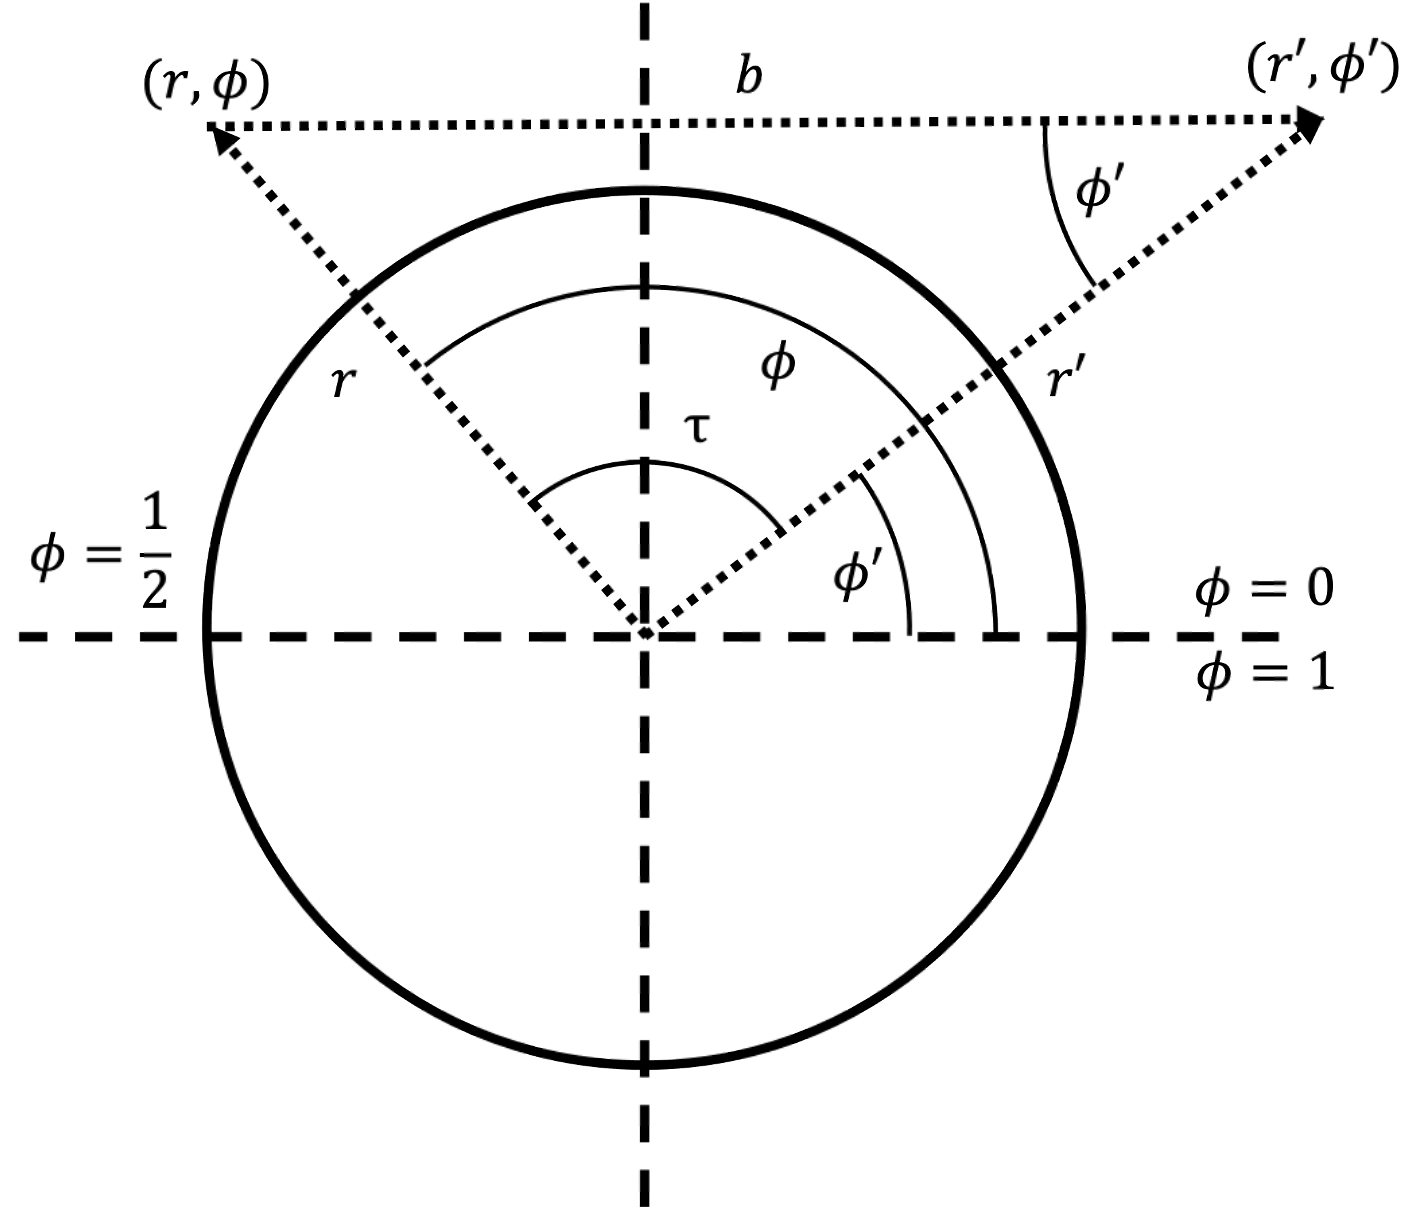
\includegraphics[width=0.45\textwidth]{../plots/Fig3.png}\label{fig:a}}
    \medskip
    \subfloat[]{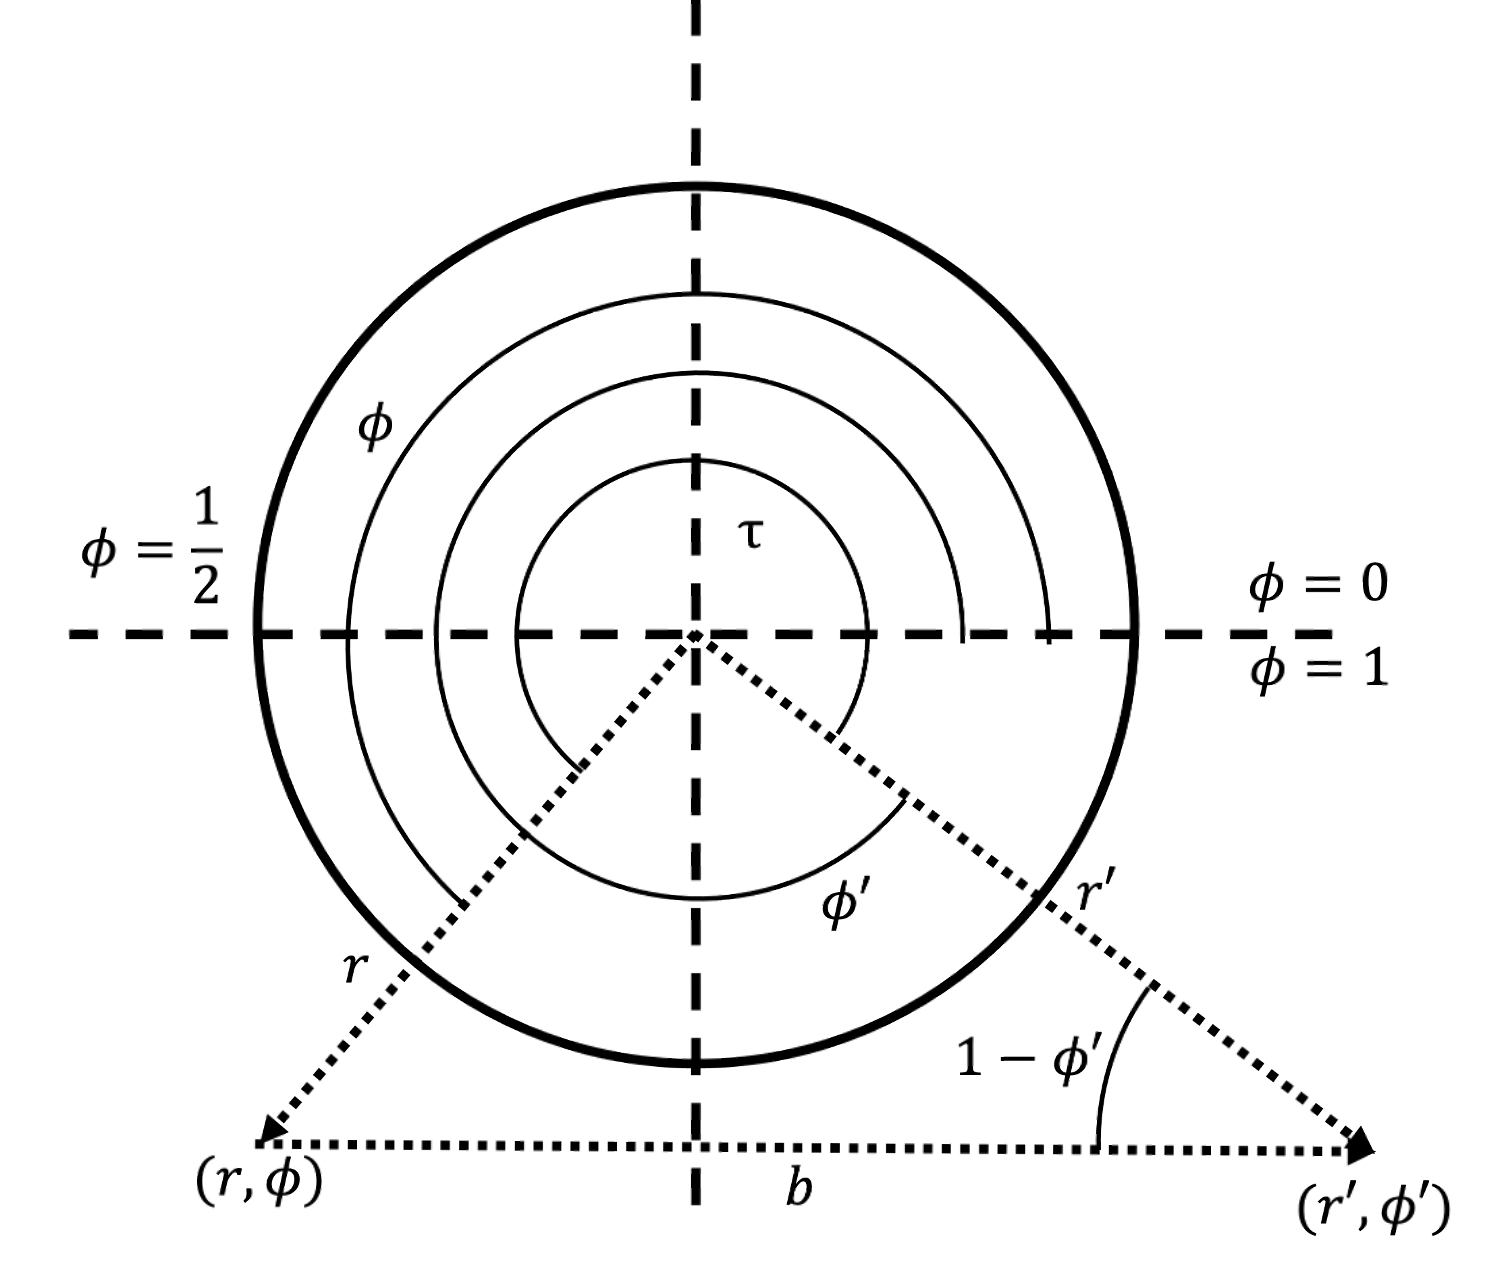
\includegraphics[width=0.45\textwidth]{../plots/Fig3-2.png}\label{fig:b}}
    \caption{\textbf{For the period-1 cycle, we can write $\tau = \phi_i - \phi'_i$ for $0\leq \phi \leq1/2$ and $\tau = 1-(\phi'_i - \phi_i)$ for $1/2\leq \phi \leq1$. Fig a) Fig b)}}
    \label{sines}
\end{figure}

\indent In order to proceed, we refer to the geometry of the period-1 cycle. Referring to Fig. \ref{sines}, the law of sines gives $\frac{\sin(2\pi \tau)}{b}=\frac{\sin(2\pi \phi'_i)}{r_i}=\frac{\sin(2\pi (\phi_i -\tau))}{r_i}$ for $0\leq \phi \leq1/2$ and $\frac{\sin(2\pi \tau)}{b}=\frac{\sin(2\pi (1-\phi'_i))}{r_i}=-\frac{\sin(2\pi \phi'_i)}{r_i}=-\frac{\sin(2\pi (1+\phi_i-\tau))}{r_i}=-\frac{\sin(2\pi (\phi_i-\tau))}{r_i}$ for $1/2\leq \phi \leq1$. Note $r_i=1$ for $k\rightarrow \infty$. This can be used to simplify:
\begin{align}
    2\pi(\phi_i - \tau) &= \arcsin(\sqrt{\frac{-b^2+4}{3b^2}}) \nonumber \\
    \pm\frac{\sin(2\pi \tau)}{b} &= \sin(\arcsin(\sqrt{\frac{-b^2+4}{3b^2}}))\nonumber \\
    (\pm\frac{\sin(2\pi \tau)}{b})^2 &= \frac{-b^2+4}{3b^2} \nonumber \\
    b &= \sqrt{4-3\sin^2(2\pi\tau)} 
    \label{eq:bound2}
\end{align}

In the Appendix section \ref{supp: sub2}, we check if there are any restrictions on $\tau$ for which $b = \sqrt{4-3\sin^2(2\pi\tau)}$ is not a period-1 instability boundary. We find $b = \sqrt{4-3\sin^2(2\pi\tau)}$ holds true only for $1/4<\tau<3/4$.\\

Furthermore, we numerically simulate the period-1 instability boundary and overlay it with the phase-locking zones (see Fig. \ref{p1-instab}). 

\begin{figure}[H]
    \begin{center}
    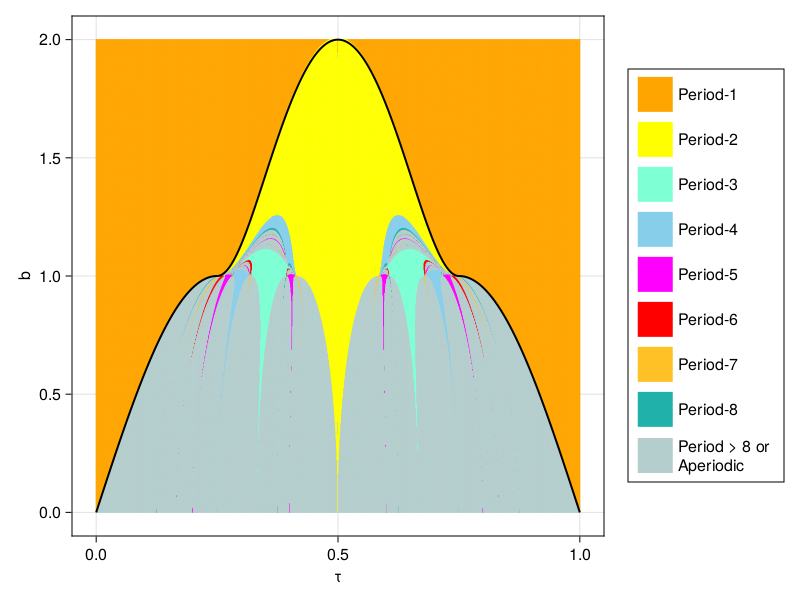
\includegraphics[width=.8\textwidth]{../plots/big_plot_w_line.png}
    \end{center}
    \caption{Phase-locking zones for the oscillator, $k=50$, with $k\rightarrow \infty$ period-1 instability boundaries $b = |\sin(2\pi\tau)|$ ($\tau \leq 1/4$, $\tau \geq 3/4$) and $b = \sqrt{4-3\sin^2(2\pi\tau)}$ ($1/4<\tau<3/4$) in black. The grey region labelled aperiodic could include stable cycles of period nine or greater, or truly aperiodic dynamics.}
    \label{p1-instab}
\end{figure}

Figure \ref{p1-instab} compares the analytically calculated period-1 instability boundaries with numerical simulations results from Section \ref{sec: Numerical Methods}. We observe quantitative agreement between period-1 instability boundaries determined by both methods, taking into consideration the domain restrictions on $\tau$ for Eq. \ref{eq:bound1} and Eq. \ref{eq:bound2}. However, it should be noted that these calculations do not reveal the cycle number for either instability boundary.

\section{Conclusion}

Periodic rhythms are fundamental in driving certain biological processes. Understanding the complex dynamics arising from periodic perturbations using a simple mathematical model is an important first step towards understanding the underlying physiology in oscillatory cardiac tissue, which in turn may eventually lead to improved treatments for diseases involving rhythmic dis-regulation.

We successfully replicated the dynamics observed by Glass \& Sun \supercite{GLASS1994} of a periodically forced Poincaré oscillator model. Specifically, the geometry of the phase-locking regions for varying stimulus intensities, time interval between stimulations, and rate of return to the limit cycle, is reproduced numerically. In addition, the period-1 instability boundary in the immediate relaxation limit is calculated analytically and is found to agree with both our numerical results and the results presented in the original study by Glass \& Sun \supercite{GLASS1994}. We clarify the mathematical origin of domain restrictions on $\tau$ for Eq. \ref{eq:bound1} and Eq. \ref{eq:bound2}. This is significant because without accounting for domain restrictions on $\tau$, analytic calculations would predict certain instability boundaries that do not exist.
